%!TEX root = ../../main.tex
\section{Proposed Solution}
Having proposed the hypothesis to solve inter-organization data sharing and transmission through secure channels, the implementation of the system is shown in this section.

\subsubsection{System technologies}
The system gathers different technologies for the simulation 

\begin{figure}[!h]
    \centering
    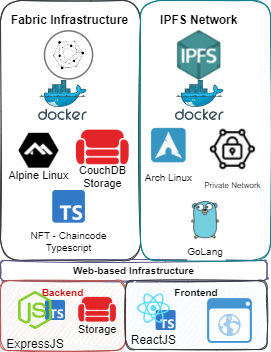
\includegraphics[scale=0.5]{img/System-Technologies.png}
    \caption{System technologies used}
    \label{fig:SystemTechUSed}
\end{figure}

\begin{itemize}
    \item \textbf{Docker}. Set of platform as a service products that use OS-level virtualization to deliver software in packages called containers.
    \item \textbf{Hyperledger Fabric version 2.2} is used in the system. It uses Docker technology to run and simulate the system. it uses \textbf{Alpine Linux} as the \ac{OS} repository.
    \item \textbf{Typescript}. A programming language superset of JavaScript developed and maintained by Microsoft. This code was used to develop the chaincode, back-end and front-end systems.
    \item \textbf{ExpressJS}. Back-end web application framework for Node.js designed for building web applications and APIs.
    \item \textbf{React}. Open-source front-end JavaScript library for building user interfaces based on UI components.
    \item \textbf{IPFS}. Decentralized file storage system used content-addressed capabilities.
    \item \textbf{Apache CouchDB}. NoSQL document-oriented open-source database.
    \item \textbf{\ac{IPFS}} Decentralized file storage system used content-addressed capabilities configured as a private network. It has been built in \textbf{GO} language and  \textbf{Alpine Linux} as \ac{OS}. Uses \textbf{Docker} containers as a base image.
\end{itemize}


\subsubsection{Proposed architecture}
The components configured and assembled to integrate the infrastructure work in a Docker system.

\begin{figure}[!h]
    \centering
    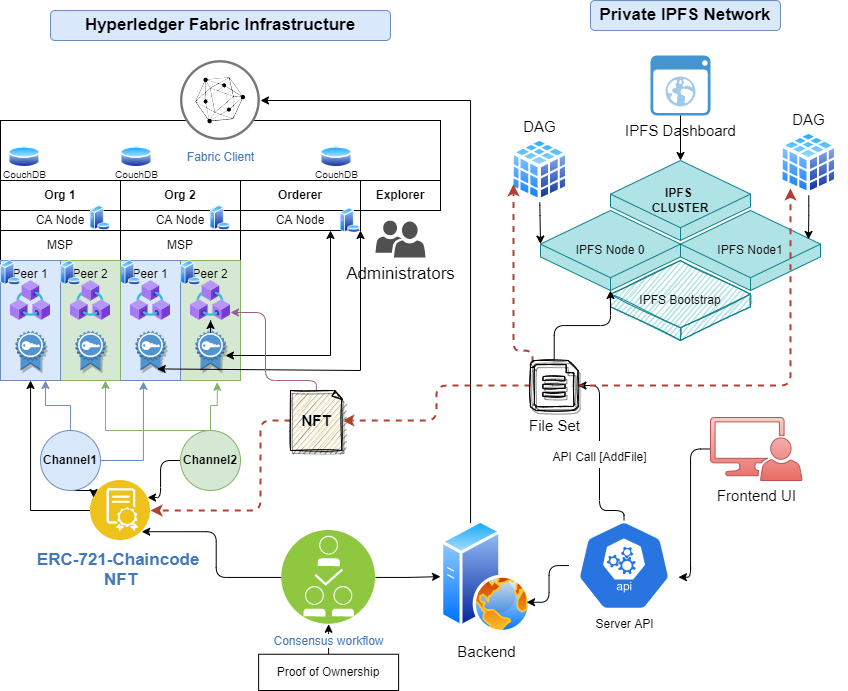
\includegraphics[width=15cm]{img/Hyperledger-NFT-Architecture.png}
    \caption{Proposed Architecture}
    \label{fig:SystemArch}
\end{figure}

\begin{itemize}
    \item \textbf{Hyperledger Fabric}. A a set of shell scripts and docker files assemble the required infrastructure to build the  \ac{DLT}. The Fabric infrastructure has the following subcomponents: 
    \begin{enumerate}
        \item Organizations. Two organizations have been created. One organizations is build primarily to simulate the minting process of a \ac{NFT} whereas the other can receive the minted token. The same process can also be made in the opposite way.
        \item Orderer node. Is the node in charge of sorting the transaction and creating the block. Once the block is created, it is forwarded to one of the organizations holding the Blockchain ledger. The orderer node does not hold a copy of the ledger but just coordinates and distributes the issued transactions.
        \item Orderer \ac{CA}. Is the node in charge of issuing and validating the certificates of the organizations and the wallet creation (based on the root certificates) for the users to interact with the system.
        \item Channel. Organizations in Hyperledger can join and interact through a private channel. The channel is previously known by the two organizations and they participate by having a server that holds a version of the ledger, a database server and a certificate authority server.
        \item Chaincode. The smart contract used to manage the ledger transaction and mint digital assets as \ac{NFT}s. The chaincode can be found in the appendix \ref{ERC271ChainCode}.
    \end{enumerate}
    \item \textbf{Private \ac{IPFS} network}. Consists of a set of Docker containers where each system holds a copy of the \ac{IPFS} file system.
    \begin{itemize}
        \item \ac{IPFS} bootstrap node. In the same way as the Ordered node receives the blocks of a transaction and transmits it to the organization nodes, it receives the file or data and transmits it to all the interconnected nodes, ensuring data persistence among the network.
        \item \ac{IPFS} Dashboard. It works as the \ac{UI} of the private network. Provides insights and data about the stored files and a preview of the data once a user can access through its content.
        \item \ac{IPFS} Nodes. Each organization can contribute to the system data repository by holding an \ac{IPFS} server.
    \end{itemize}
    \item \textbf{Back-end}. Server application that communicates with the Hyperledger network and extends its functionality by an API. 
    \begin{itemize}
        \item Connects organizations and corporate databases
        \item Communicates with the \ac{CA} servers to issue and hold certificates.
        \item Communicates with \ac{IPFS} private network API. 
        \item Holds a public \ac{REST} \ac{API} that provides all the functionality to register organizations, enroll users and mint \ac{NFT}s.
        \item Interacts with the Blockchain smart contract and retrieves the information contained in the ledger. 
    \end{itemize}
    \item \textbf{Front-end}. It serves as the \ac{UI} for user interaction. Allows the simulation of the system where any user can create an organization, enroll users, mint a \ac{NFT} and visualize them in the list.
\end{itemize}